\documentclass[a4paper, 12pt, onecolumn]{book}

\usepackage{helvet}
\usepackage[slovak]{babel}
\usepackage[utf8]{inputenc}
\usepackage[T1]{fontenc}
\usepackage{lmodern}
\usepackage{graphicx}
\usepackage{amsmath, amsthm, amsfonts}
\usepackage[table]{xcolor}
\usepackage[absolute,overlay]{textpos}
\usepackage{csvsimple}
\usepackage{tabularx}
\usepackage{array}
\usepackage[margin=0cm]{geometry}
\usepackage{datatool}
\DTLsetseparator{,}

\renewcommand{\familydefault}{\sfdefault}
\begin{document}

\thispagestyle{empty}										% Odstráni číslo strany	

\definecolor{profiyellow}{rgb}{1.0, 0.87, 0.0}
\definecolor{silver}{rgb}{0.75, 0.75, 0.75}
\definecolor{dimgray}{rgb}{0.41, 0.41, 0.41}

%% ============================== VARIABLES ============================== %% 
\name=name
\marking=marking
\variantscount=3
\newcommand{\path}{}

%% ============================== TOP and BOTTOM ============================== %%
\begin{figure}[t!]
	
\includegraphics[width=\paperwidth]{top.pdf}
\end{figure}


\begin{figure}[b!]
	
\includegraphics[width=\paperwidth]{bottom.pdf}
\end{figure} 

%% ============================== NAME ============================== %% 
\begin{textblock*}{10cm}(10cm, 0.7cm) 	% {block width} (coords) 
	\centering
  {\fontsize{30}{0} \selectfont \textbf{ \name }}
\end{textblock*}

%% ============================== IMAGE ============================== %% 
\begin{textblock*}{7cm}(1cm, 3.5cm)
	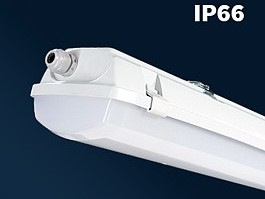
\includegraphics[width=7cm]{img.jpg}
\end{textblock*}

\begin{textblock*}{7cm}(1cm, 11cm)
	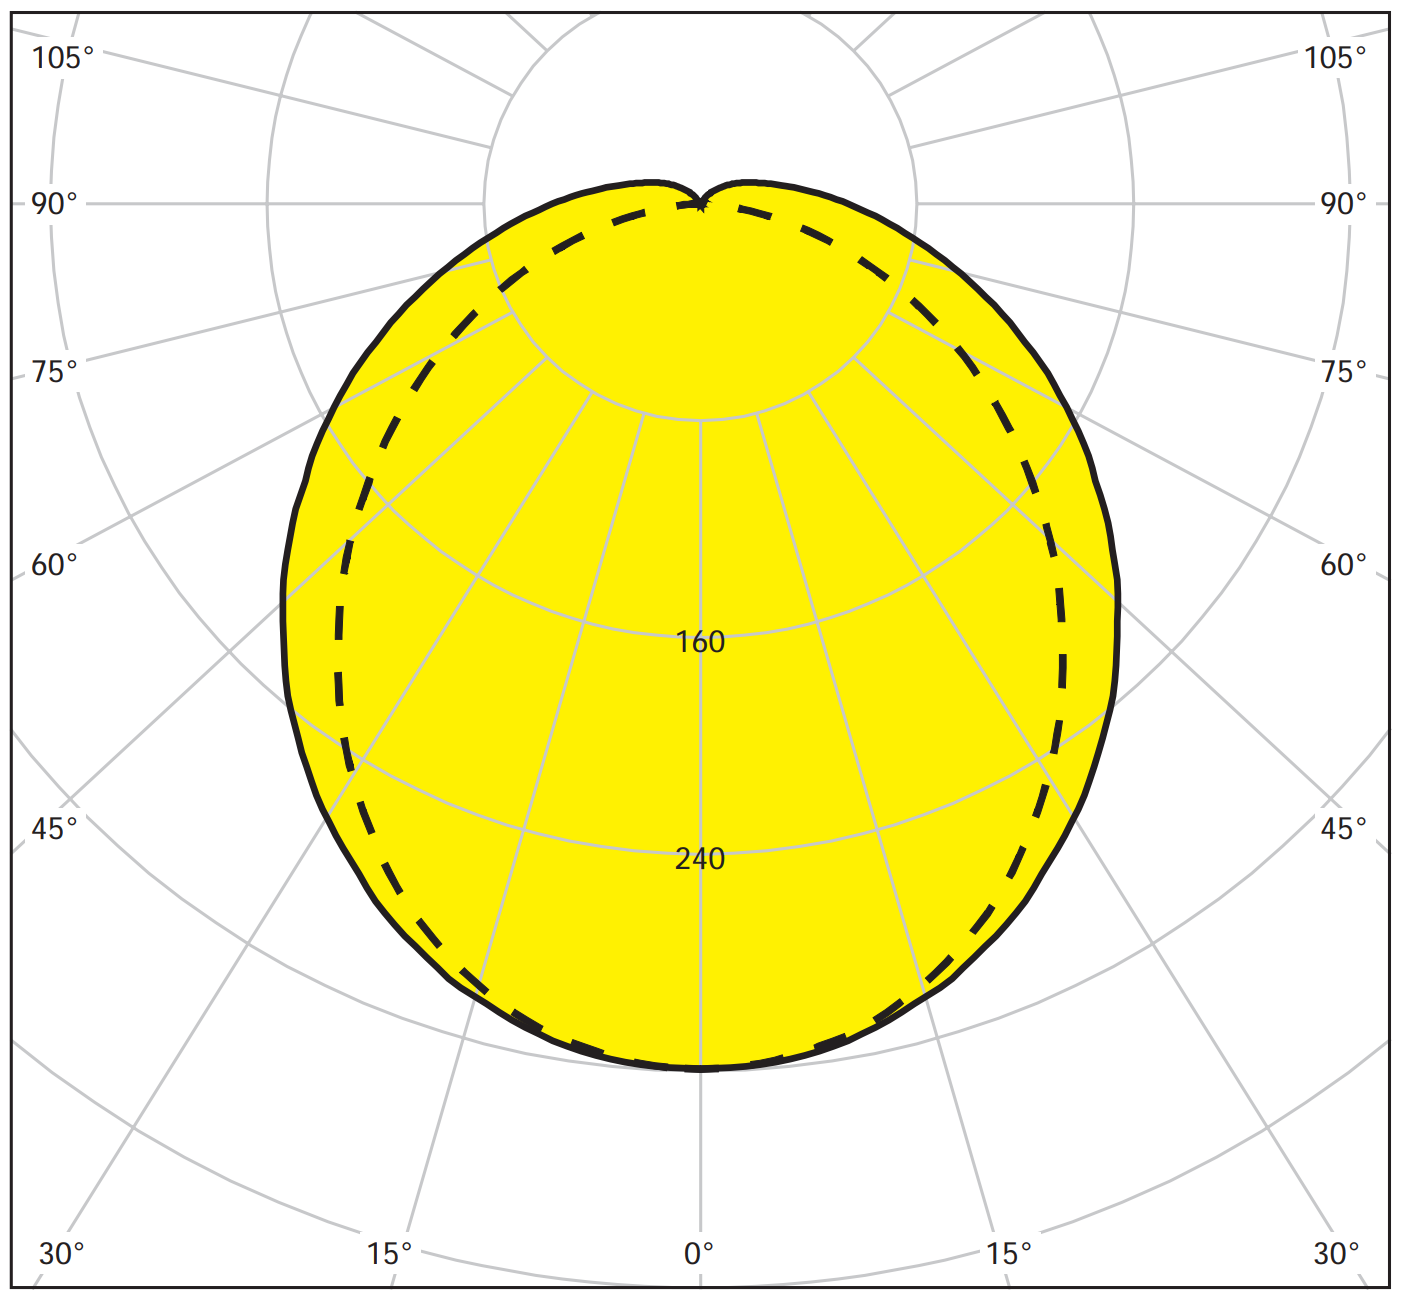
\includegraphics[width=7cm]{curve.PNG}
\end{textblock*}

%% ============================== TABLE of DATA ============================== %%
\setlength{\arrayrulewidth}{0.3mm}
\setlength{\extrarowheight}{0.3cm}

\begin{textblock*}{11cm}(10cm, 3.5cm) 												% {block width} (coords)
{\rowcolors{3}{gray!10}{white}
	\begin{tabularx}{9cm}{l  X}
\rowcolor{dimgray}\multicolumn{2}{c}{\textbf{\color{white}Vlastnosti svietidla}} \\
\hline
\textbf{Označenie:} & ANC-LED \\ 
\textbf{Popis:} & Prachotes do priemyselných priestorov. \\ 
\textbf{Montáž:} & SUR \\ 
\textbf{Optika:} & PMMA difúzor \\ 
\textbf{Materiál:} & plast \\ 
\textbf{Krytie IP:} & 66 \\ 
\textbf{Krytie IK:} & 10 \\ 
\textbf{Index podania farieb:} & >80 \\ 
\textbf{Tolerancia sv. toku:} & +-10 \\ 
\textbf{Pracovná teplota:} & Od -20 do +30 \\ 
\textbf{Životnosť:} & L50B70 50 000 \\ 
\textbf{Možnosti:} & DALI \\ 
\end{tabularx}
}
\end{textblock*}

%% ============================== TABLE of VARIANTS ============================== %%
\setlength{\arrayrulewidth}{0.3mm}
\setlength{\extrarowheight}{1mm}

\begin{textblock*}{18cm}(1.5cm, 20cm) 								% {block width} (coords)
	\centering
	{\rowcolors{3}{profiyellow}{profiyellow!50}
		\begin{tabularx}{\textwidth}{X || *{6}{c}}
\rowcolor{white}\multicolumn{7}{c}{\textbf{Dostupné varianty}} \\
\hline
\rowcolor{dimgray}
\textcolor{white}{Kód} & \textcolor{white}{Výkon} & \textcolor{white}{Svietivosť} & \textcolor{white}{CCT} & \textcolor{white}{Výška} & \textcolor{white}{Priemer} & \textcolor{white}{Hmotnosť} \\ 
\hline
- & [W] & [lm] & [K] & [mm] & [mm] & [kg] \\ 
\hline\hline
AXIMA-24-3 & 24 & 2150 & 3000 & 95 & 390 & 1.7 \\ 
AXIMA-24-4 & 24 & 2300 & 4000 & 95 & 390 & 1.7 \\ 
\end{tabularx}
	}
\end{textblock*}


\end{document}
